\documentclass[11pt,a4paper]{article}
\usepackage[utf8]{inputenc}
\usepackage[T1]{fontenc}
\usepackage{lmodern}
\usepackage[margin=2.2cm]{geometry}
\usepackage{graphicx}
\usepackage{booktabs}
\usepackage{float}
\usepackage{xcolor}
\usepackage{amsmath}
\usepackage{caption}
\usepackage{enumitem}
\usepackage[hidelinks]{hyperref}
\graphicspath{{../../figures/}{./}}

\definecolor{navy}{HTML}{1B2A4A}
\definecolor{amber}{HTML}{B5650F}
\newcommand{\var}[1]{\texttt{\detokenize{#1}}}
\newenvironment{reading}{\par\smallskip\noindent\textbf{\color{navy}Interpretation.}\ }{\par\medskip}
\setlist{itemsep=2pt,topsep=3pt}
\captionsetup{font=small,labelfont=bf}
\widowpenalty=10000 \clubpenalty=10000
\setlength{\parskip}{4pt}\setlength{\parindent}{0pt}

\title{\textbf{Cross-Network Intrusion Analysis}\\[4pt]
\large Phase 4 --- Exploratory Data Analysis of the merged NetFlow data}
\author{Ahmed Hamouda}
\date{Notebook \texttt{07\_eda\_netflow.ipynb}}

\begin{document}
\maketitle

\section{Data and method}

\textbf{Data.} The merged NetFlow v3 table produced in phase 3 combines four networks: UNSW-NB15 (mixed lab network),
CSE-CIC-IDS2018 (enterprise office network), ToN-IoT (IoT / industrial network) and BoT-IoT (IoT botnet network).
It contains \textbf{17,551,848 rows standing for 63,012,224 flows}.

\textbf{Unit of analysis: the behaviour.} During cleaning, identical flows were merged into one row with a
\var{count} column. Every statistic and test counts \emph{behaviours} (rows): identical copies of a flow are not
independent observations, and counting them would let the large floods dominate every result.

\textbf{Research questions addressed.}
\begin{itemize}
  \item \textbf{SQ1:} which traffic characteristics distinguish normal traffic from attack traffic?
  \item \textbf{SQ2:} does the same attack family behave the same way in different networks?
\end{itemize}

\textbf{Key variables.} Four variables describe a flow: \var{IN_BYTES} (bytes sent by the client),
\var{OUT_BYTES} (bytes sent back), \var{IN_PKTS} (packets sent) and \var{FLOW_DURATION_MILLISECONDS} (duration).
The correlation analysis uses 12 traffic features.

\textbf{Full data or sample.} Counts, summary statistics, histograms and the Mann--Whitney test use \emph{all}
17.5 million rows. Box plots, correlation heatmaps and the Kolmogorov--Smirnov test use \emph{one} stratified sample:
up to 10,000 random behaviours from each network $\times$ family group (187,418 rows, \texttt{random\_state = 42}).
Without it, Benign would fill two thirds of every plot and the smallest family (448 behaviours) would be invisible.

\section{First look at the data}

\begin{table}[H]\centering\small
\caption{Behaviours (rows) per family and network.}
\begin{tabular}{lrrrrr}
\toprule
Family & UNSW & CIC-2018 & ToN-IoT & BoT-IoT & All \\
\midrule
Benign & 1,307,351 & 8,178,232 & 2,282,642 & 21,951 & 11,790,176 \\
Denial of service & 5,360 & 642,600 & 573,277 & 642,187 & 1,863,424 \\
Reconnaissance & 13,134 & -- & 225,074 & 898,728 & 1,136,936 \\
Credential attacks & -- & 94,890 & 697,124 & -- & 792,014 \\
Web and injection & -- & 53 & 1,831,103 & -- & 1,831,156 \\
Malware and botnets & 3,802 & 2,804 & 23,471 & -- & 30,077 \\
Exploitation and intrusion & 42,740 & 27,213 & -- & -- & 69,953 \\
Interception and spoofing & -- & -- & 4,951 & -- & 4,951 \\
Fuzzing and crypto & 32,713 & -- & -- & -- & 32,713 \\
Data theft & -- & -- & -- & 448 & 448 \\
\midrule
All behaviours & 1,405,100 & 8,945,792 & 5,637,642 & 1,563,314 & 17,551,848 \\
All flows & 2,350,609 & 19,285,037 & 24,442,770 & 16,933,808 & 63,012,224 \\
\bottomrule
\end{tabular}
\end{table}

\begin{figure}[H]\centering
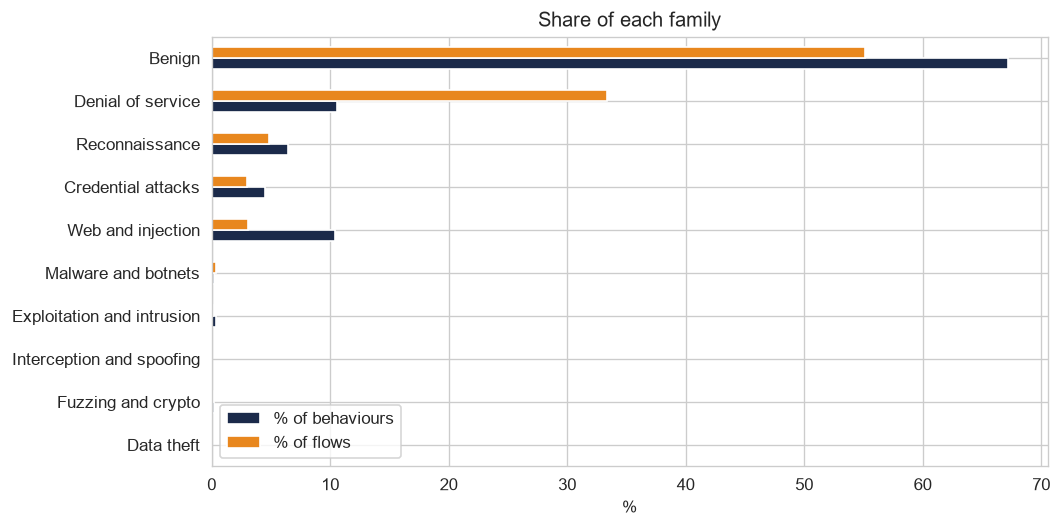
\includegraphics[width=0.7\linewidth]{NetFlow_eda_families.png}
\caption{Share of each family in behaviours and in flows.}
\end{figure}

\begin{reading}
\begin{itemize}
  \item The data are complete: \textbf{no missing value}.
  \item \textbf{Benign is the majority} with 67\% of the behaviours. Denial of service (11\%) and Web and injection
        (10\%) are the largest attack families; Data theft has only 448 behaviours.
  \item \textbf{Behaviours versus flows:} Denial of service is 11\% of the behaviours but 33\% of the flows, because a
        flood repeats the same flow many times. Counting behaviours prevents floods from dominating the analysis.
  \item \textbf{Not every family exists in every network.} Only Benign and Denial of service are present in all four.
        Fuzzing comes only from UNSW, Interception only from ToN-IoT, Data theft only from BoT-IoT, and Web and
        injection practically only from ToN-IoT. Comparisons across networks (SQ2) are therefore made on Denial of
        service.
\end{itemize}
\end{reading}

\section{Summary statistics}

\begin{table}[H]\centering\small
\caption{Summary statistics of the key variables (all 17.5 million behaviours).}
\begin{tabular}{lrrrrrrr}
\toprule
Variable & Mean & Median & Std & Q1 & Q3 & IQR & Skewness \\
\midrule
\var{IN_BYTES} & 3,725 & 701 & 142,790 & 164 & 1,623 & 1,459 & 357.2 \\
\var{OUT_BYTES} & 11,338 & 940 & 315,030 & 127 & 2,239 & 2,112 & 194.5 \\
\var{IN_PKTS} & 32.9 & 6 & 1,664 & 3 & 10 & 7 & 179.4 \\
\var{FLOW_DURATION_MILLISECONDS} & 14,549 & 755 & 33,205 & 47 & 4,057 & 4,010 & 2.4 \\
\bottomrule
\end{tabular}
\end{table}

\begin{reading}
All four variables are \textbf{strongly right-skewed}.
\begin{itemize}
  \item The mean is much larger than the median (\var{IN_BYTES}: 3,725 against 701 bytes), because a few huge flows
        pull the mean up; the largest carries 189\,MB.
  \item The skewness is far above 1 (357 for \var{IN_BYTES}), the limit above which a variable is ``highly skewed''.
  \item The standard deviation is larger than the mean.
\end{itemize}
The \textbf{median and the IQR} therefore describe a typical flow better than the mean and the standard deviation.
A typical behaviour sends 701 bytes in 6 packets and lasts 0.75\,s. The duration never exceeds 121\,s, because the
NetFlow exporter cuts longer connections into pieces.
\end{reading}

\begin{table}[H]\centering\small
\caption{Median of the key variables per family (all behaviours).}
\begin{tabular}{lrrrr}
\toprule
Family & \var{IN_BYTES} & \var{OUT_BYTES} & \var{IN_PKTS} & Duration (ms) \\
\midrule
Benign & 1,135 & 1,572 & 8 & 1,325 \\
Denial of service & 528 & 1,136 & 6 & 10,812 \\
Reconnaissance & 44 & 40 & 1 & 23 \\
Credential attacks & 481 & 2,142 & 6 & 438 \\
Web and injection & 760 & 1,304 & 6 & 304 \\
Malware and botnets & 288 & 240 & 6 & 1,506 \\
Exploitation and intrusion & 822 & 555 & 10 & 800 \\
Interception and spoofing & 140 & 258 & 2 & 37 \\
Fuzzing and crypto & 812 & 336 & 10 & 708 \\
Data theft & 1,658 & 3,380 & 14 & 2,407 \\
\bottomrule
\end{tabular}
\end{table}

\begin{reading}
Each family has its own typical flow:
\begin{itemize}
  \item \textbf{Reconnaissance} is the smallest (44 bytes, 1 packet, 23\,ms): a single probe packet, typical of a scan.
  \item \textbf{Denial of service} lasts the longest (median 10.8\,s): connections held open or flooded.
  \item \textbf{Data theft} moves the most data (1,658 bytes sent, 3,380 received, 14 packets).
  \item \textbf{Interception and spoofing} is short and small (140 bytes, 37\,ms), like DNS messages.
\end{itemize}
The traffic variables therefore carry information about the type of attack (SQ1).
\end{reading}

\section{Plots of one variable}

\begin{figure}[H]\centering
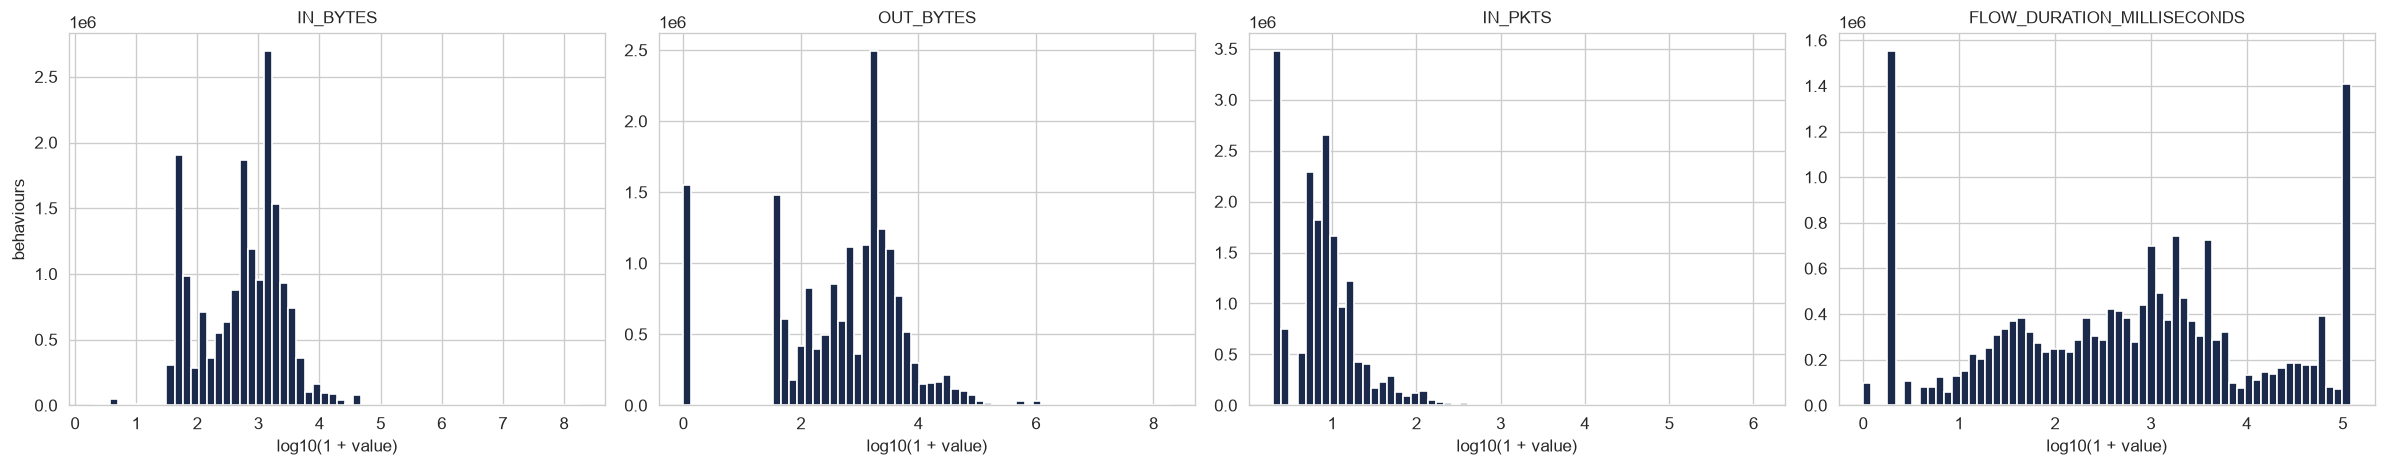
\includegraphics[width=\linewidth]{NetFlow_eda_histograms.png}
\caption{Histograms of the key variables, all behaviours. The axis shows $\log_{10}(1+\text{value})$: each step of 1
means $\times 10$ (2 = 100, 3 = 1,000), and the ``+1'' keeps the zeros on the plot.}
\end{figure}

\begin{reading}
None of the variables has a bell shape, even on a log scale. The distributions have several peaks and tall spikes at
single values, each with a technical cause:
\begin{itemize}
  \item \var{OUT_BYTES} $= 0$ for 8.8\% of the behaviours: \textbf{no answer} (a scan of a closed port, a flooded victim);
  \item \var{IN_PKTS} $= 1$: one-packet flows (probes, DNS queries);
  \item \var{FLOW_DURATION_MILLISECONDS} piles up near 0\,ms and at 120\,s (the exporter's time limit).
\end{itemize}
These shapes already suggest that normality will be rejected (Section~7.1).
\end{reading}

\begin{figure}[H]\centering
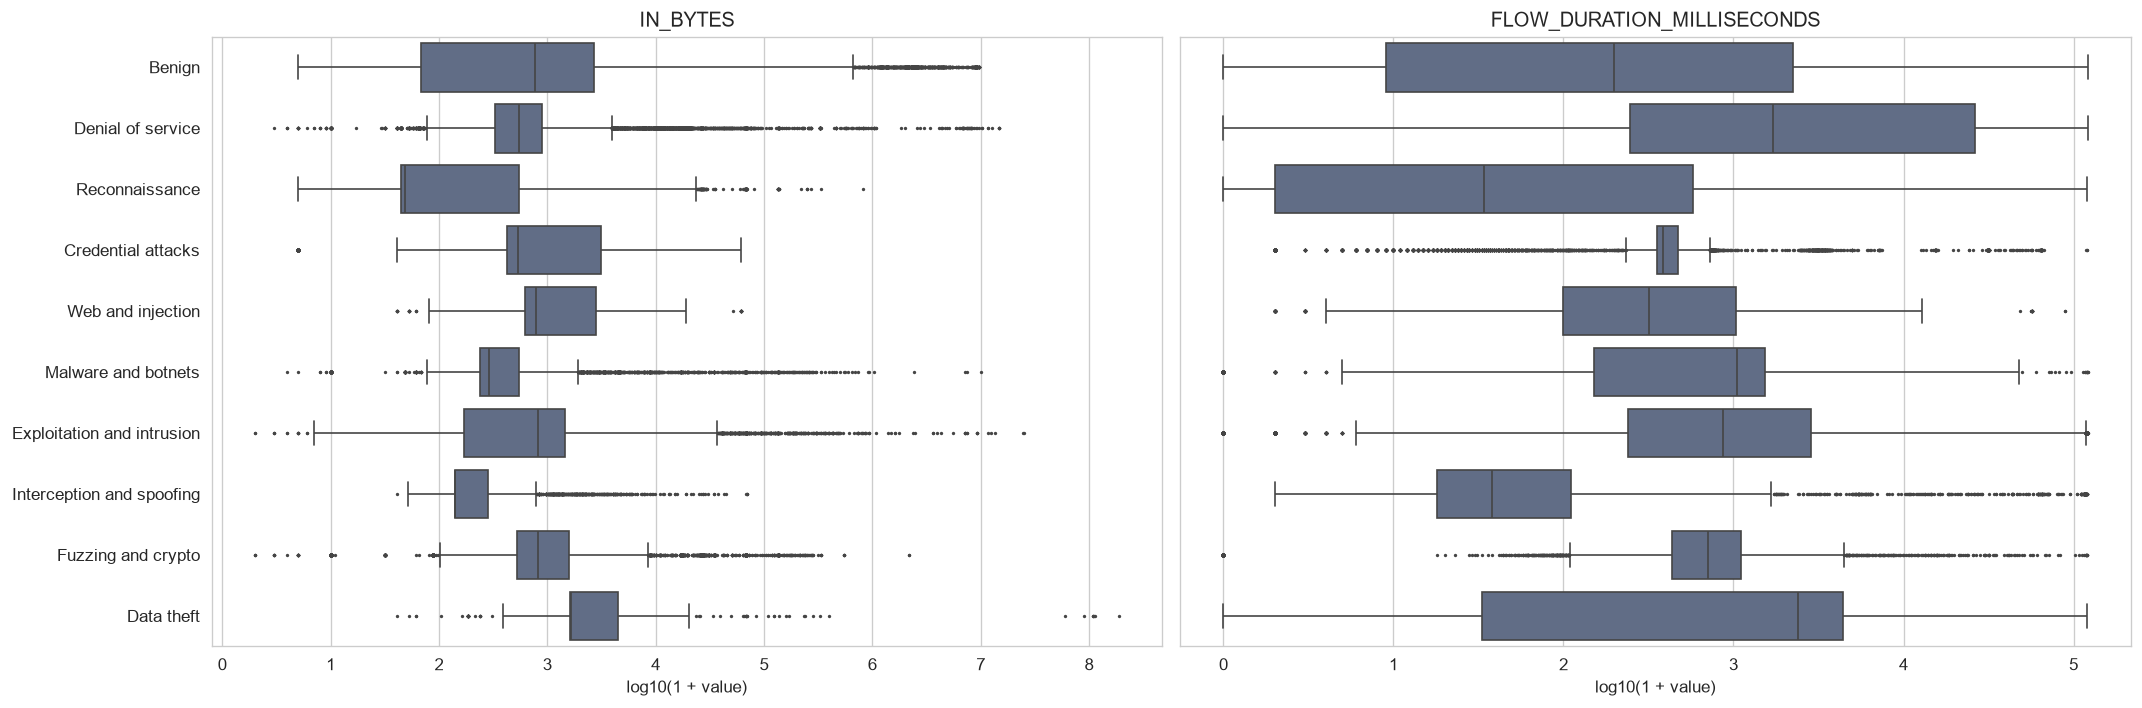
\includegraphics[width=\linewidth]{NetFlow_eda_boxplots_by_family.png}
\caption{Box plots by family (stratified sample, log scale). Middle line = median, box = Q1 to Q3.}
\end{figure}

\begin{reading}
The families are clearly shifted from each other: Reconnaissance has the smallest byte counts and the shortest flows,
Denial of service the longest flows, Data theft the most bytes. However, \textbf{the Benign box covers almost the whole
range of the attack families}: no single variable separates normal traffic from all attacks, so a detection model
will need several variables together. The points beyond the whiskers are mostly real attacks (large floods, long
connections) and are kept.
\end{reading}

\section{Correlation analysis}

\begin{figure}[H]\centering
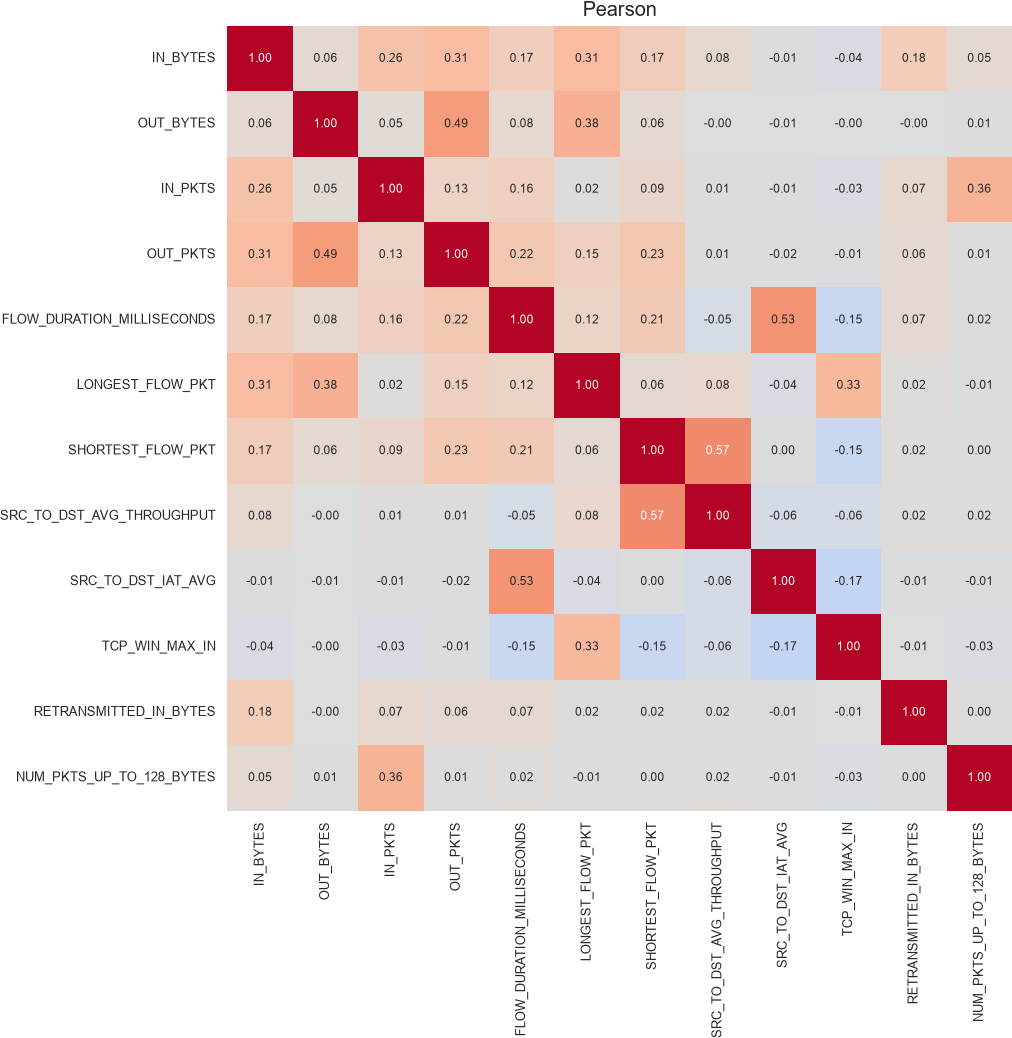
\includegraphics[width=0.6\linewidth]{corr_pearson.png}
\caption{Pearson correlation of 12 traffic features (stratified sample).}
\end{figure}

\begin{figure}[H]\centering
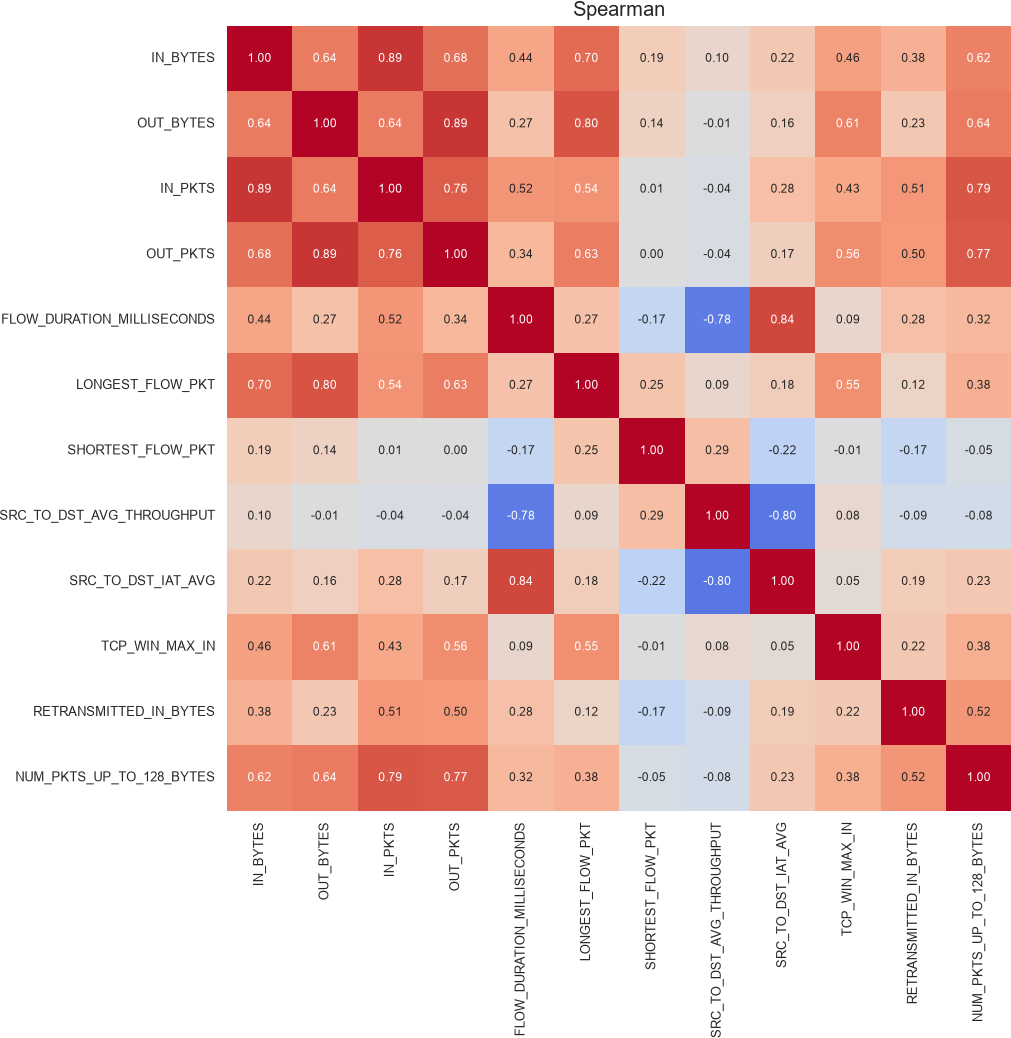
\includegraphics[width=0.6\linewidth]{corr_spearman.png}
\caption{Spearman correlation of the same 12 features (stratified sample).}
\end{figure}

\begin{table}[H]\centering\small
\caption{Pairs where Pearson and Spearman disagree most, and the strongest Spearman pairs.}
\begin{tabular}{llrr}
\toprule
Variable 1 & Variable 2 & Pearson $r$ & Spearman $\rho$ \\
\midrule
\var{IN_BYTES} & \var{IN_PKTS} & 0.26 & 0.89 \\
\var{OUT_PKTS} & \var{NUM_PKTS_UP_TO_128_BYTES} & 0.01 & 0.77 \\
\var{SRC_TO_DST_AVG_THROUGHPUT} & \var{SRC_TO_DST_IAT_AVG} & $-0.06$ & $-0.80$ \\
\var{FLOW_DURATION_MILLISECONDS} & \var{SRC_TO_DST_AVG_THROUGHPUT} & $-0.05$ & $-0.78$ \\
\var{OUT_BYTES} & \var{OUT_PKTS} & 0.49 & 0.89 \\
\var{FLOW_DURATION_MILLISECONDS} & \var{SRC_TO_DST_IAT_AVG} & 0.53 & 0.84 \\
\var{OUT_BYTES} & \var{LONGEST_FLOW_PKT} & 0.38 & 0.80 \\
\bottomrule
\end{tabular}
\end{table}

\begin{reading}
The two heatmaps look very different. Pearson measures straight-line relationships and finds almost none, because a
few gigantic flows dominate it. Spearman works on ranks, is not affected by extreme values, and finds strong
relationships (for example \var{IN_BYTES}--\var{IN_PKTS}: $r = 0.26$ but $\rho = 0.89$). \textbf{Spearman is the right
coefficient for this data.} The main relationships are:
\begin{itemize}
  \item \textbf{volume:} bytes and packets rise together ($\rho = 0.89$ in both directions), and the more data a flow
        carries, the larger its biggest packet ($\rho = 0.80$);
  \item \textbf{time:} longer flows have longer gaps between packets ($\rho = 0.84$) and a lower throughput
        ($\rho = -0.78$).
\end{itemize}
Strongly correlated columns carry similar information; feature selection in phase 5 will keep one of each group.
\end{reading}

\section{Relationships between variables}
\subsection{Benign versus attack traffic in each network}

\begin{figure}[H]\centering
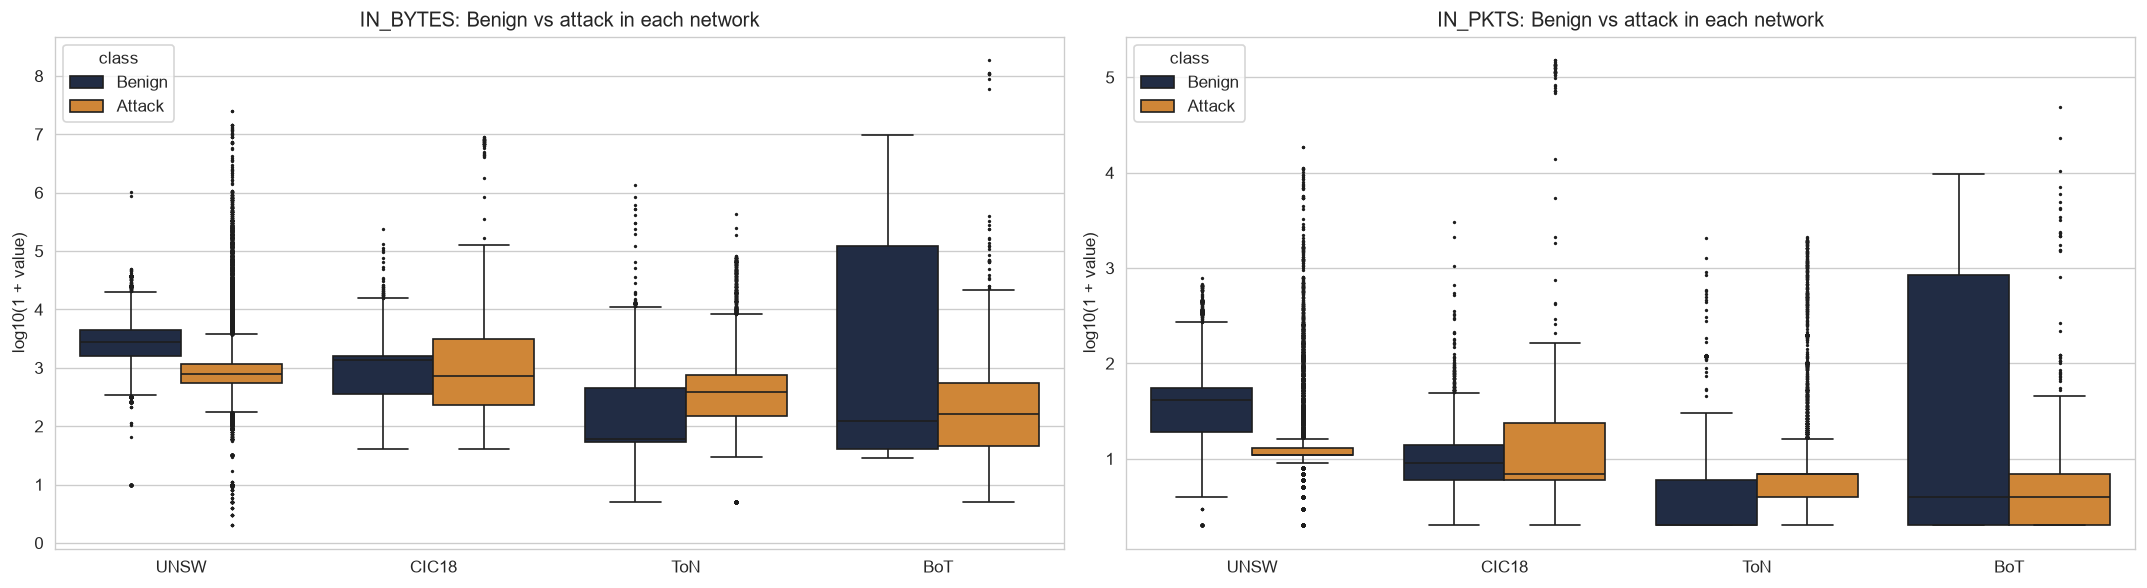
\includegraphics[width=\linewidth]{NetFlow_eda_benign_vs_attack.png}
\caption{Bytes and packets sent, Benign against attack, in each network (stratified sample, log scale).}
\end{figure}

\begin{table}[H]\centering\small
\caption{Median of the key variables, Benign against attack, per network (all behaviours).}
\begin{tabular}{lrrrrrrrr}
\toprule
& \multicolumn{2}{c}{\var{IN_BYTES}} & \multicolumn{2}{c}{\var{OUT_BYTES}} & \multicolumn{2}{c}{\var{IN_PKTS}} & \multicolumn{2}{c}{Duration (ms)} \\
\cmidrule(lr){2-3}\cmidrule(lr){4-5}\cmidrule(lr){6-7}\cmidrule(lr){8-9}
Network & Benign & Attack & Benign & Attack & Benign & Attack & Benign & Attack \\
\midrule
UNSW & 2,750 & 814 & 8,824 & 336 & 40 & 10 & 95 & 716 \\
CIC-2018 & 1,369 & 510 & 1,873 & 1,147 & 8 & 5 & 2,845 & 3,334 \\
ToN-IoT & 65 & 637 & 52 & 1,155 & 1 & 6 & 22 & 377 \\
BoT-IoT & 120 & 44 & 40 & 40 & 3 & 1 & 31 & 51 \\
\bottomrule
\end{tabular}
\end{table}

\begin{reading}
This is the most important relationship of the analysis: \textbf{the difference between Benign and attack traffic is
not the same in every network; it even points in opposite directions.}
\begin{itemize}
  \item \textbf{UNSW:} attacks are \emph{smaller} than normal traffic (814 against 2,750 bytes, 10 against 40 packets).
  \item \textbf{ToN-IoT:} attacks are \emph{larger} (637 against 65 bytes, 6 against 1 packet), because ToN-IoT's
        normal traffic consists mostly of tiny one-packet flows.
  \item \textbf{CIC-2018 and BoT-IoT:} the two classes are close.
\end{itemize}
Normal traffic itself differs strongly between networks (40 packets in UNSW, 1 in ToN-IoT). A rule such as ``attacks
send more bytes'' holds in one network and fails in another. Test~1 (Section~7.2) checks this formally.
\end{reading}

\subsection{Destination port range and family}

\begin{figure}[H]\centering
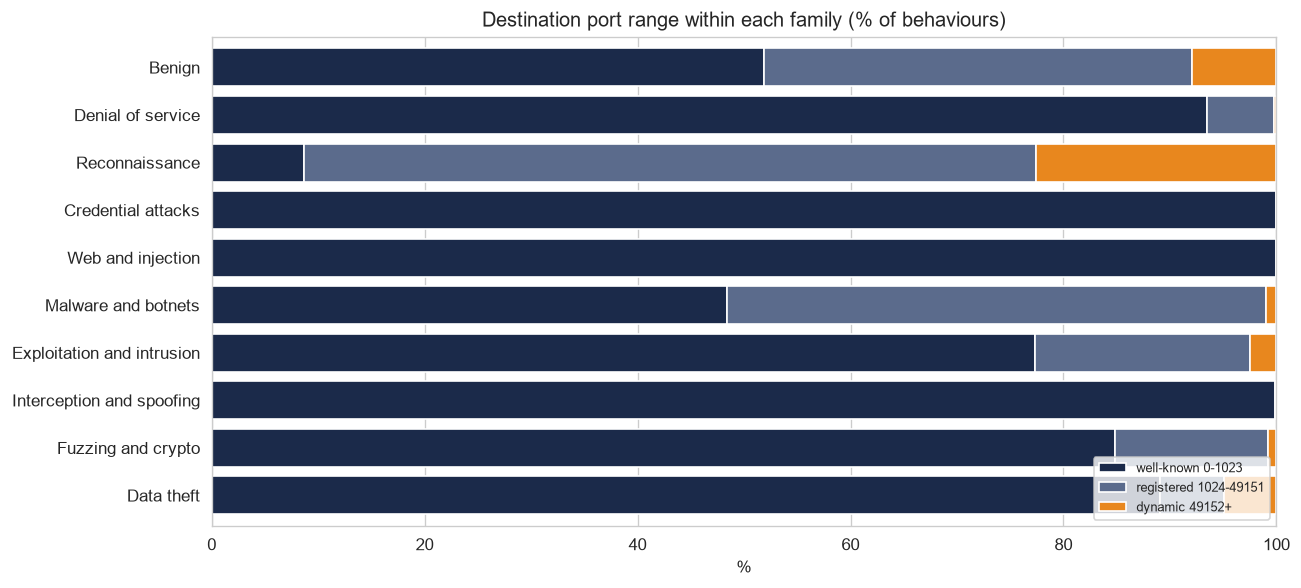
\includegraphics[width=0.8\linewidth]{NetFlow_eda_port_range_by_family.png}
\caption{Destination port range within each family (\% of behaviours, all data). Well-known 0--1023 = standard
services (80 HTTP, 22 SSH, 53 DNS); registered 1024--49151; dynamic 49152--65535.}
\end{figure}

\begin{table}[H]\centering\small
\caption{Destination port range per family (row \%).}
\begin{tabular}{lrrr}
\toprule
Family & Well-known & Registered & Dynamic \\
\midrule
Benign & 51.9 & 40.1 & 8.0 \\
Denial of service & 93.5 & 6.3 & 0.2 \\
Reconnaissance & 8.7 & 68.8 & 22.5 \\
Credential attacks & 99.9 & 0.1 & 0.0 \\
Web and injection & 100.0 & 0.0 & 0.0 \\
Malware and botnets & 48.4 & 50.6 & 1.0 \\
Exploitation and intrusion & 77.4 & 20.2 & 2.4 \\
Interception and spoofing & 99.9 & 0.1 & 0.0 \\
Fuzzing and crypto & 84.8 & 14.5 & 0.7 \\
Data theft & 89.1 & 6.0 & 4.9 \\
\bottomrule
\end{tabular}
\end{table}

\begin{reading}
The port range is strongly linked to the family.
\begin{itemize}
  \item Web, Credential, Interception and Denial-of-service traffic goes almost only to \textbf{well-known ports}
        (93--100\%): these attacks target standard services.
  \item \textbf{Reconnaissance} goes 91\% to registered and dynamic ports: a scan tries many ports, whereas a real
        service uses a few known ones.
  \item \textbf{Benign} traffic is mixed (52\% well-known, 40\% registered).
\end{itemize}
The destination port is therefore a useful variable for recognising the type of attack (SQ1); it will be encoded as a
category in phase 5.
\end{reading}

\section{Hypothesis tests}
\subsection{Normality check: which kind of test can be used?}

The t-test and ANOVA assume roughly normal data. Shapiro--Wilk and D'Agostino--Pearson test
\textbf{H$_0$: the data come from a normal distribution}, on 5,000 random behaviours (the limit of Shapiro--Wilk), on
the raw values and after $\log(1+x)$.

\begin{table}[H]\centering\small
\caption{Normality tests (5,000 random behaviours from the sample).}
\begin{tabular}{llrrrc}
\toprule
Variable & Scale & Skewness & Shapiro--Wilk $p$ & D'Agostino $p$ & Normal? \\
\midrule
\var{IN_BYTES} & raw & 18.95 & $2\times10^{-94}$ & $<10^{-300}$ & no \\
 & $\log(1+x)$ & 1.10 & $3\times10^{-44}$ & $3\times10^{-238}$ & no \\
\var{OUT_BYTES} & raw & 25.16 & $1\times10^{-94}$ & $<10^{-300}$ & no \\
 & $\log(1+x)$ & $-0.36$ & $4\times10^{-43}$ & $9\times10^{-37}$ & no \\
\var{IN_PKTS} & raw & 48.85 & $2\times10^{-95}$ & $<10^{-300}$ & no \\
 & $\log(1+x)$ & 1.89 & $4\times10^{-57}$ & $<10^{-300}$ & no \\
\var{FLOW_DURATION_MILLISECONDS} & raw & 3.85 & $1\times10^{-84}$ & $<10^{-300}$ & no \\
 & $\log(1+x)$ & $-0.14$ & $2\times10^{-32}$ & $2\times10^{-22}$ & no \\
\bottomrule
\end{tabular}
\end{table}

\begin{figure}[H]\centering
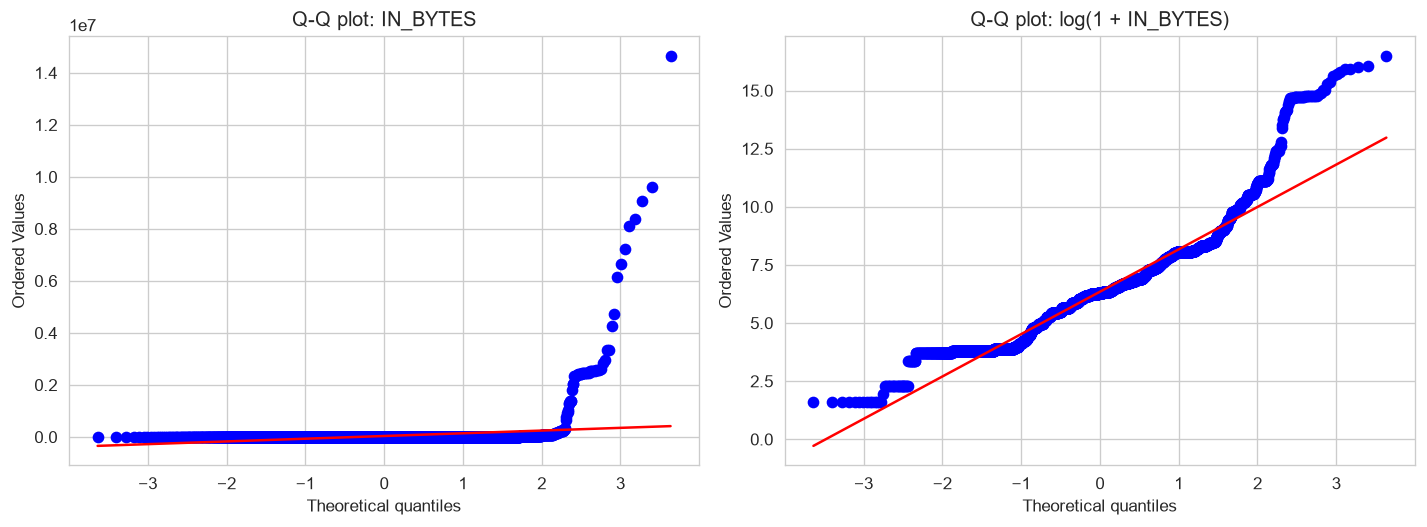
\includegraphics[width=0.8\linewidth]{NetFlow_eda_normality_qq.png}
\caption{Q-Q plots of \var{IN_BYTES}, raw (left) and $\log(1+x)$ (right). Points on the line would mean a normal
distribution.}
\end{figure}

\begin{reading}
Visually, no variable follows the normal curve. On the raw scale the Q-Q points lie flat along the bottom and then
shoot up (a few huge values). After $\log(1+x)$ they come closer to the line but form a \textbf{staircase}, because
many flows share exactly the same value. Both formal tests reject normality for every variable on both scales (all
p-values below $10^{-20}$). With 5,000 values the tests would also catch small, harmless departures, but here the
departures are large: the raw skewness is between 4 and 49, and the plots show it clearly. The log transform helps the
shape (\var{IN_BYTES} skewness 19 to 1.1) but does not make the data normal.

\textbf{Practical conclusion:} the t-test and ANOVA, which compare means and assume normal groups, are not suitable.
The tests below use the \textbf{non-parametric} alternatives from the Chapter 4 slides, which work on ranks and need
no normality. The CICIoT2023 analysis reached the same conclusion.
\end{reading}

\textbf{How the tests are read.} With hundreds of thousands of rows, even a tiny difference gives $p \approx 0$. The
p-value says \emph{whether} there is a difference; the \textbf{effect size} says \emph{how large} it is, and the
conclusion rests on it. Because several tests answer the same question, p-values are multiplied by the number of tests
(\textbf{Bonferroni correction}) before being compared with $\alpha = 0.05$.

\subsection{Test 1 (SQ1) --- Mann--Whitney U: does attack traffic differ from Benign traffic?}

\textbf{Effect sizes used.}
\begin{itemize}
  \item Rank-biserial $r = \frac{2U}{n_1 n_2} - 1 \in [-1, 1]$: $r > 0$ means attacks are larger, $r < 0$ smaller.
        $|r| < 0.1$ negligible, $< 0.3$ small, $< 0.5$ medium, $\geq 0.5$ large.
  \item In plain words, $P(\text{attack} > \text{Benign}) = (1 + r)/2$ is the chance that a random attack behaviour is
        larger than a random Benign behaviour (ties counted half); 50\% means no difference.
  \item The 95\% confidence interval of the difference in medians uses the distribution-free interval of each median
        (the sorted values at ranks $n/2 \pm 1.96\sqrt{n}/2$), which needs no normality.
\end{itemize}

\begin{table}[H]\centering\small
\caption{Mann--Whitney U: effect size $r$ (attack against Benign) for the 16 tests.}
\begin{tabular}{lrrrr}
\toprule
Variable & UNSW & CIC-2018 & ToN-IoT & BoT-IoT \\
\midrule
\var{IN_BYTES} & $-0.50$ & $-0.11$ & $+0.51$ & $-0.10$ \\
\var{OUT_BYTES} & $-0.73$ & $+0.04$ & $+0.69$ & $-0.13$ \\
\var{IN_PKTS} & $-0.62$ & $-0.11$ & $+0.59$ & $-0.22$ \\
\var{FLOW_DURATION_MILLISECONDS} & $+0.46$ & $-0.05$ & $+0.36$ & $+0.12$ \\
\midrule
Effect & large & negligible--small & large & small \\
\bottomrule
\end{tabular}
\end{table}

\begin{table}[H]\centering\footnotesize\setlength{\tabcolsep}{4pt}
\caption{One example per network: medians, 95\% confidence interval of the difference, and effect sizes.}
\begin{tabular}{llcrrl}
\toprule
Network & Variable & Median attack vs Benign (95\% CI of diff.) & $r$ & $P(\text{att.} > \text{Ben.})$ & Effect \\
\midrule
UNSW & \var{OUT_BYTES} & 336 vs 8,824 bytes ($-8{,}488$ to $-8{,}488$) & $-0.73$ & 14\% & large, smaller \\
ToN-IoT & \var{OUT_BYTES} & 1,155 vs 52 bytes ($+1{,}098$ to $+1{,}106$) & $+0.69$ & 84\% & large, larger \\
CIC-2018 & \var{IN_BYTES} & 510 vs 1,369 bytes ($-861$ to $-858$) & $-0.11$ & 45\% & small \\
BoT-IoT & \var{IN_PKTS} & 1 vs 3 packets ($-2$ to $-2$) & $-0.22$ & 39\% & small \\
\bottomrule
\end{tabular}
\end{table}

\begin{reading}
\begin{itemize}
  \item \textbf{H$_0$:} in each network, attack and Benign behaviours have the same distribution of the variable.
        \textbf{H$_1$:} the distributions differ.
  \item \textbf{Assumptions checked and test chosen (why):} the two groups are different behaviours, so they are
        independent. Normality is rejected (Section~7.1), so the two-sample t-test is not suitable and its rank-based
        alternative, the Mann--Whitney U test, is used. It runs on all behaviours of each network (from 21,951 to
        8,178,232 per group).
  \item \textbf{Test and p-value:} 16 tests (4 networks $\times$ 4 variables); for example UNSW \var{OUT_BYTES}:
        $U = 1.75\times10^{10}$, $p < 10^{-300}$. All 16 Bonferroni-corrected p-values are below $10^{-180}$.
  \item \textbf{Decision ($\alpha = 0.05$):} reject H$_0$ in all 16 tests.
  \item \textbf{Conclusion in plain language:} the size and the direction of the difference depend on the network.
        \begin{itemize}
          \item In UNSW, a random attack flow receives more data than a random Benign flow only 14\% of the time.
          \item In ToN-IoT, it does so 84\% of the time.
          \item In CIC-2018 and BoT-IoT, the effects are small.
        \end{itemize}
        The confidence intervals are very narrow because they use millions of behaviours: the medians are known almost
        exactly. Two cases show why the whole distribution matters, not only the median:
        \begin{itemize}
          \item in CIC-2018, \var{OUT_BYTES} has a lower median for attacks but $r$ is slightly positive (+0.04),
                because the two distributions cross; the effect is negligible either way;
          \item in BoT-IoT, the confidence interval of the duration difference includes 0 ($-88$ to $+32$\,ms): the
                medians may be equal, yet the test finds a small difference in the distributions ($r = +0.12$).
        \end{itemize}
\end{itemize}
\textbf{Answer to SQ1:} attack traffic does differ from normal traffic, often strongly, but \textbf{which variable shows
it and in which direction depends on the network}. A rule learned in one network (``attacks are small'') can be wrong
in another.
\end{reading}

\subsection{Test 2 (SQ2) --- Kolmogorov--Smirnov: does the same family behave the same way in every network?}

\textbf{Family tested:} Denial of service, the only attack family present in all four networks.
\textbf{Effect size:} $D$ = the largest gap between the two cumulative curves, from 0 (identical) to 1 (no overlap);
$D < 0.1$ practically the same, $0.1$--$0.3$ moderately different, $> 0.3$ clearly different.

\begin{table}[H]\centering\small
\caption{Kolmogorov--Smirnov on Denial of service (12 tests; all Bonferroni-corrected $p < 10^{-68}$).}
\begin{tabular}{lrrrr}
\toprule
& \multicolumn{2}{c}{\var{IN_BYTES}} & \multicolumn{2}{c}{Duration} \\
\cmidrule(lr){2-3}\cmidrule(lr){4-5}
Pair of networks & $D$ & Medians (bytes) & $D$ & Medians (ms) \\
\midrule
UNSW vs CIC-2018 & 0.49 & 814 / 485 & 0.51 & 651 / 8,889 \\
UNSW vs ToN-IoT & 0.15 & 814 / 874 & 0.26 & 651 / 443 \\
UNSW vs BoT-IoT & 0.48 & 814 / 420 & 0.95 & 651 / 28,749 \\
CIC-2018 vs ToN-IoT & 0.48 & 485 / 874 & 0.59 & 8,889 / 443 \\
CIC-2018 vs BoT-IoT & 0.21 & 485 / 420 & 0.51 & 8,889 / 28,749 \\
ToN-IoT vs BoT-IoT & 0.54 & 874 / 420 & \textbf{0.99} & 443 / 28,749 \\
\bottomrule
\end{tabular}
\end{table}

\begin{figure}[H]\centering
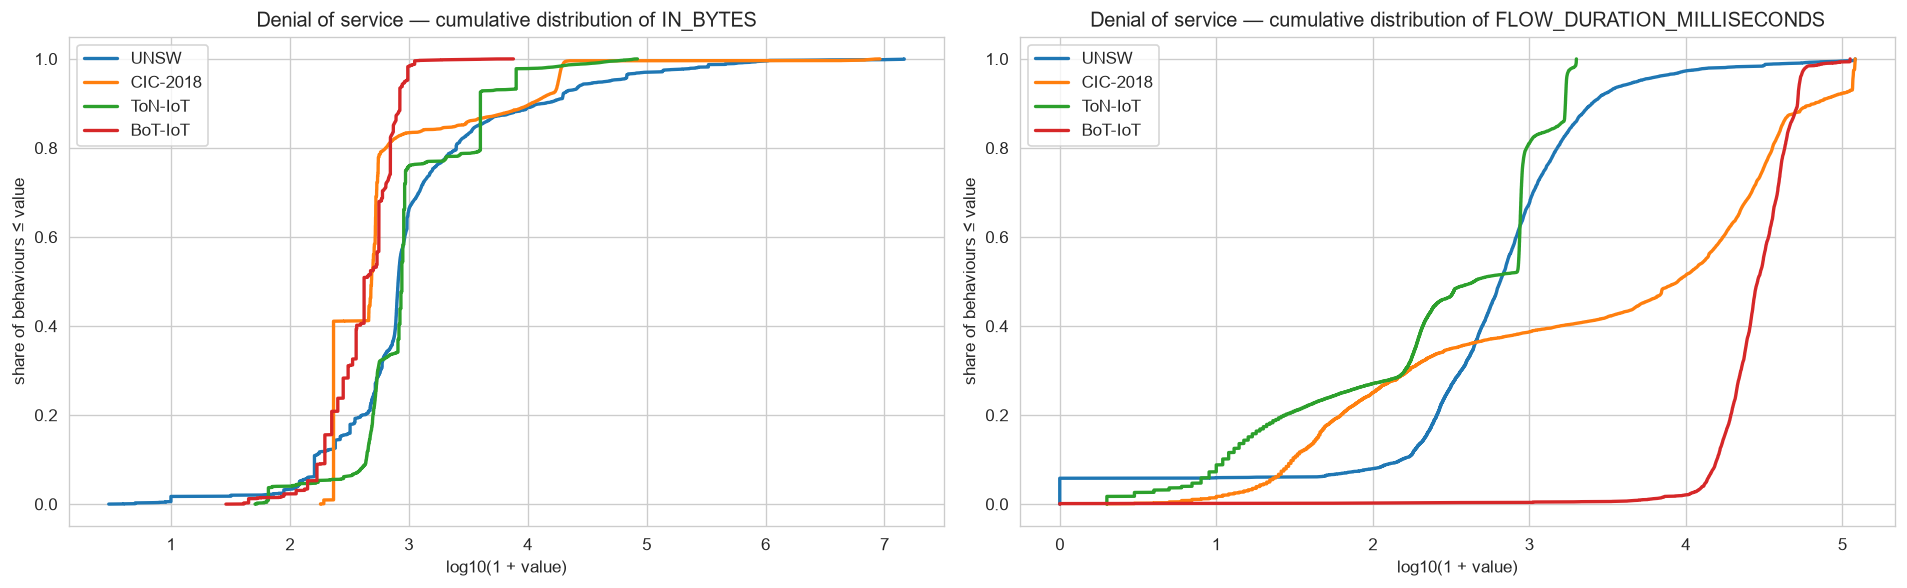
\includegraphics[width=0.85\linewidth]{NetFlow_eda_ks_dos.png}
\caption{Denial of service: cumulative distribution of bytes and duration in each network. Identical behaviour would
make the four curves lie on top of each other.}
\end{figure}

\begin{reading}
\begin{itemize}
  \item \textbf{H$_0$:} Denial-of-service flows have the same distribution in the two networks. \textbf{H$_1$:} the
        distributions differ.
  \item \textbf{Assumptions checked and test chosen (why):} the two samples come from different networks, so they are
        independent. Normality is rejected (Section~7.1). The question is whether the whole behaviour is the same, not
        only the centre, so the two-sample Kolmogorov--Smirnov test is used: it compares the complete cumulative
        distributions. 6 pairs of networks $\times$ 2 variables = 12 tests, with up to 10,000 behaviours per network.
  \item \textbf{Test and p-value:} largest effect ToN-IoT vs BoT-IoT on the duration, $D = 0.99$, $p < 10^{-300}$;
        smallest effect UNSW vs ToN-IoT on the bytes, $D = 0.15$, $p = 3\times10^{-69}$. All 12 Bonferroni-corrected
        p-values are below $10^{-68}$.
  \item \textbf{Decision ($\alpha = 0.05$):} reject H$_0$ in all 12 tests.
  \item \textbf{Conclusion in plain language:} a denial-of-service flow lasts a median of \textbf{0.4\,s in ToN-IoT}
        but \textbf{29\,s in BoT-IoT}; with $D = 0.99$ the two distributions barely overlap. Of the 12 comparisons,
        9 are clearly different ($D > 0.3$), 3 moderately different and none the same. The cumulative curves of the
        four networks are far apart instead of lying on top of each other.
\end{itemize}
\textbf{Answer to SQ2:} the same attack family does \textbf{not} produce the same traffic in different networks. The
testbeds used different tools, victims and settings, and these change the flows more than the attack type keeps them
alike.
\end{reading}

\section{Wrap-up: what did the exploration tell us?}

\textbf{Three most important findings.}
\begin{enumerate}
  \item \textbf{SQ1:} attack traffic differs from normal traffic, but the direction depends on the network. In UNSW,
        attacks are smaller than Benign traffic ($r$ down to $-0.73$); in ToN-IoT they are larger ($r$ up to $+0.69$).
        No single variable separates attacks from normal traffic everywhere.
  \item \textbf{SQ2:} the same attack family does not behave the same way in different networks. Denial of service
        lasts a median of 0.4\,s in ToN-IoT and 29\,s in BoT-IoT (KS $D = 0.99$), and none of the 12 comparisons finds
        the same distribution.
  \item \textbf{The families have different profiles:} one-packet scans, long denial-of-service connections, large
        data-theft transfers. The destination port range is strongly linked to the family (scans use high ports, web
        and credential attacks use well-known ports). The variables do carry information about the type of attack.
\end{enumerate}

\textbf{Data-quality caveat.} The traffic is far from normal (strong skewness, many repeated technical values such as
the exporter's 120\,s time limit). Some differences between networks therefore come from how each testbed was built
and recorded, not only from the attacks. Because the data are so large, every p-value is close to 0, so the
conclusions rest on the effect sizes ($r$, $D$).

\textbf{Follow-up question.} No single variable separates attacks from normal traffic in all four networks. Can a
\textbf{combination} of variables do it, and how much accuracy is lost on a network the model has never seen (SQ3)?

\textbf{Next steps (phase 5).}
\begin{itemize}
  \item Log-transform the volume and time variables.
  \item Encode the destination port as a category.
  \item Keep one variable from each strongly correlated group.
\end{itemize}

\end{document}
